\section{Formalização}

\label{section:formalizacao}

Nesta seção vamos formalizar o modelo HAIL através de um modelo de cascata, partindo dos conceitos mais gerais e afunilando para as definições mais específicas e fórmulas matemáticas utilizadas. Para isso, começamos com uma única tupla que define de maneira geral o que é o modelo que se desdobra para os demais conceitos. O objetivo disso é criar camadas de abstração, as quais podem ser modificadas de acordo com a necessidade de implementações específicas ou da integração com arquiteturas cognitivas ou outros modelos.

 O bloco básico do modelo de revisão de percepções proposto, chamado de HAIL, é composto por um módulo para alucinação e ilusão $M_{ai}$ e uma função de refinamento $\theta$, conforme descrito na Definição \ref{def:modeloHAIL}. O módulo de ilusão e alucinação é uma quádrupla, apresentada na definição \ref{def:illuHallu}. A função de refinamento é uma função abstrata, cuja entrada é obtida através dos sensores do agentes e a saída é a entrada do módulo de alucinação e ilusão, conforme já foi descrito anteriormente na Seção \ref{refinamento}.
 
 \begin{definition}{}
    O modelo de revisão de percepções HAIL é uma dupla $HAIL = \langle M_{ai}, \theta \rangle$, onde:
    
    \begin{itemize}
        \item $M_{ai}$ é o módulo de ilusão e alucinação; e
        \item $\theta$ é a função de refinamento $\theta(p) = \rho$, onde $p$ é um conjunto de percepções e $\rho$ é um subconjunto próprio de $p$.
    \end{itemize}{}
    \label{def:modeloHAIL}
\end{definition}

Após ter passado pela função $\theta$, as percepções $\rho$ irão passar pelo Algoritmo \ref{algorithm:decisor}, e serão encaminhadas de acordo com sua classificação. O bloco de ilusão e alucinação é descrito por uma quádrupla, com conjuntos de decisores, blocos e uma função de transição.

\begin{definition}
\label{def:illuHallu}
    O bloco de ilusão e alucinação é uma quádrupla $M_{ai} = \langle D, Ab, Ap, \Delta \rangle$, onde:
    
    \begin{itemize}
        \item $D$ é o conjunto de decisores $D = \{d_{a}, d_{h}, d_{i}\}$, onde:
             \begin{itemize}
                \item $d_{a}$ é o decisor de anomalias, definido pela função:
                \[ d_{a} = \left\{ \begin{array}{ll}
                0 & \mbox{se $\rho(x)$ está em $c$\footnotemark};\\
                1 & \mbox{se $\rho(x)$ não está em $c$}.\end{array} \right. \]
             
                \item $d_{h}$ é o decisor de alucinação, definido pela função:
                \[ d_{h} = \left\{ \begin{array}{ll}
                0 & \mbox{se nem $\rho$ nem $(x)$ está em $c$};\\
                1 & \mbox{se $\rho$ ou $(x)$ está em $c$}.\end{array} \right. \]
                
                \item $d_{i}$ é o decisor de ilusão, definido pela função:
                \[ d_{i} = \left\{ \begin{array}{ll}
                0 & \mbox{se $\rho$ está em $c$};\\
                1 & \mbox{se $(x)$ está em $c$}.\end{array} \right. \]
            \end{itemize}
        
        \footnotetext{ $c$ é o contexto do agente, de acordo com a definição \ref{definition::context}.}
        
        \item $Ab$ é o conjunto de blocos avaliadores $Ab = \{Ab_{h}, Ab_{i1}, Ab_{i2}\}$, onde $Ab_{h}$ é o bloco avaliador de alucinações, $Ab_{i1}$ é o bloco avaliador de ilusões classe 1 e $Ab_{i2}$ é o bloco avaliador de ilusões classe 2.
        
        \item $Ap$ é o conjunto de blocos de planejamento automatizado $Ap = \{Ap_{h}, Ap_{i}\}$, onde $Ap_{h}$ é o bloco de planejamento automatizado de alucinações e $Ap_{i}$ é o bloco de planejamento automatizado de ilusões.
        
        \item $\Delta$ é a função de transição definido pela tabela abaixo, onde $out$ é um estado final, que leva a percepção para fora do modelo de revisão de percepções, ou seja, pode tanto significar o encaminhamento de uma percepção válida para o raciocínio do agente quanto o fim da execução de um ciclo de revisão.
        
            \begin{table}[htb]
                \caption{Função de transição $\Delta$ do módulo de ilusão e alucinação.}
                \centering
                \begin{tabular}{c c c c} 
                    \toprule
                    \textbf{Estado} & \textbf{0} & \textbf{1} \\
                    \midrule
                    $d_{a}$     & $out$     & $d_{h}$       \\
                    $d_{h}$     & $Ab_{h}$  & $d_{i}$       \\
                    $d_{i}$     & $Ab_{i1}$ & $Ab_{i2}$     \\
                    $Ab_{h}$    & $out$     & $Ap_{h}$      \\
                    $Ab_{i1}$   & $out$     & $Ap_{i}$      \\
                    $Ab_{i2}$   & $out$     & $Ap_{i}$      \\
                    \bottomrule
                \end{tabular}
                \label{transition-table}
                \legend{Fonte: Autor.}
                
            \end{table}
    \end{itemize}{}
\end{definition}{}

O módulo de ilusão e alucinação é o artefato principal do modelo. Ele recebe uma entrada $\rho$, que é a saída da função de refinamento apresentada na definição 1, e processa cada um dos elementos $\rho(x)$ desse conjunto, através de decisores e blocos de avaliação, percorrendo o modelo de acordo com as transições descritas pela função de transição $\Delta$. Os três decisores do conjunto $D$ fazem a triagem para detectar se a percepção $\rho(x)$ é uma anomalia, e que tipo de anomalia é. Após passar pelos três decisores, saberemos se essa percepção é valida, é uma alucinação, é uma ilusão tipo 1 ou uma ilusão tipo 2. Após ter passado pelos decisores, a percepção ou é levada para a cognição do agente, caso seja válida, ou fica armazenada nos blocos avaliadores, caso seja uma anomalia.

\begin{definition}
    Um bloco avaliador é uma tripla $Ab_{x} = \langle L, Pf, Cf) \rangle$, $x \in \{h, i1, i2\}$, onde:

    \begin{itemize}
        \item $L$ é uma lista ordenada pelo número de vezes que uma mesma anomalia é dada como entrada;
        \item $Pf$ é a função de processamento, definida abaixo:
            
             \[ Pf = \left\{ \begin{array}{ll}
                        1 & \mbox{se $T_{m}(A) \leq T_{m}(V) * (|A| - |A_{pr}|)$;}\\
                        0 & \mbox{caso contrário}.\end{array} \right. \]
        
            
            Onde:
            
            \begin{itemize}
                \item $T_{m}$ é a função que retorna a média do tempo gasto para processar as percepções de um conjunto;
                \item $A$ é o conjunto de anomalias, $A(x)$ é um elemento específico $x$ e $|A|$ o número de anomalias do conjunto;
                \item $A_{pr}$ é o conjunto de anomalias que já foram validadas para serem processadas pela função de processamento neste ciclo de raciocínio ($A_{pr}$ é instanciada vazia a cada ciclo de raciocínio), e $|A_{pr}|$ o número de anomalias desse conjunto.
                \item $V$ é o conjunto de percepções válidas.
            \end{itemize}{}
        
        \item $Cf$ é a função de limpeza definida abaixo com auxílio da função equação de limpeza $Cf$, sendo $\alpha$ um coeficiente de limpeza variável que precisa ser definido pela instância implementada do modelo (por padrão, toma-se $\alpha = 1$):
        
        \[ Cf = \left\{ \begin{array}{ll}
                        1 & \mbox{se  $Ce = Verdadeiro$;}\\
                        0 & \mbox{caso contrário}.\end{array} \right. \]
            
            \[ Ce = \sum_{i=1}^{|L|} W_{n}(L_{i}) > \alpha \sum_{j=1}^{|L|} W_{1}(L_{j}) \]
            
            Onde:
            
            \begin{itemize}
                \item $L$ é a lista ordenada do bloco, sendo $|L|$ seu número de anomalias e $L_{i}$ a anomalia $i$ da lista.
                \item $W$ é a função peso da anomalia $L_{i}$ definida como $W(L_{i}) = |L_{i}|$, sendo $|L_{i}|$ o peso da anomalia especificada (número de entradas recebidas dessa mesma anomalia na lista). A função $W$ é utilizada para especificar as seguintes funções:
                \\
                
                    (i) $ W_{1}(L_{i}) = \left\{ \begin{array}{ll}
                        1 & \mbox{se $W(L_{i}) = 1$;}\\
                        0 & \mbox{caso contrário}.\end{array} \right. $
                \\
                
                    (ii) $ W_{n}(L_{i}) = \left\{ \begin{array}{ll}
                        W(L{i}) & \mbox{se $W(L_{i}) > 1$;}\\
                        0 & \mbox{caso contrário}.\end{array} \right. $
            \end{itemize}{}
    \end{itemize}
\end{definition}{}

A terceira definição é a de bloco de avaliação ($Ab$). Um $Ab$ é um módulo do modelo que é responsável por armazenar as anomalias detectadas e decidir se elas serão processadas pelo agente ou não. É descrito por uma tripla, constituída por uma lista ordenada $L$, uma função de processamento $Pf$ e uma função de limpeza $Cf$. $L$ é uma lista organizada pela recorrência de elementos inseridos nela, onde cada elemento só aparece uma vez e contém um número de vezes que o mesmo elemento já foi inserido nela, chamado de peso. Nesse modelo, os elementos são as anomalias percebidas pelo agente, e o peso é o número de vezes que o agente percebeu a anomalia.

$Pf$ é uma função que avalia se uma anomalia será processada nesse ciclo de raciocínio ou se será armazenada para ser processada no futuro. Para isso, ela precisa de uma função que retorne o tempo médio previsto para o processamento de uma percepção $T_m$, seja ela uma percepção válida ou uma anomalia. Com base nessa função, $Pf$ retorna 1 caso o tempo médio de processamento de uma anomalia seja menor que o tempo médio de processamento de uma percepção válida multiplicado pelo número de anomalias que fazem parte desse ciclo de raciocínio menos o número de anomalias que já foram aprovadas pelo bloco avaliador, e zero caso contrário.

De maneira simplificada, o objetivo dessa função é evitar que o modelo de revisão de percepção gaste mais tempo de processamento do que ele gastaria caso não estivesse sendo utilizado e todas as percepções fossem válidas. Para isso, o bloco avaliador permite processar apenas as anomalias que aparecem de maneira mais recorrente para o agente.

$Cf$ é uma função que realiza a limpeza de $L$. Conforme os ciclos de raciocínio forem passando, $L$ tende a possuir diversas anomalias que foram percebidas apenas uma única vez. Dessa maneira, uma grande quantidade de memória seria necessária para armazenar as possíveis centenas de anomalias que podem nunca ser processadas. Assim, a função $Cf$ verifica se a equação $Ce$ é verdadeira ou falsa. Ela é verdadeira quando o número de anomalias que apareceram uma única vez é maior que a soma dos pesos das anomalias que apareceram mais de uma vez (o peso é o número atrelado a cada anomalia, que representa quantas vezes elas já foram inseridas na lista). Quando a função for verdadeira, o bloco avaliador remove todas as anomalias de peso 1 da lista.

O coeficiente de limpeza $\alpha$ presente em $Ce$ pode ser utilizado na implementação do HAIL quando é necessário que a limpeza seja mais ou menos recorrente. Por padrão, caso a instância do HAIL não queira alterar a frequência da limpeza das filas, utiliza-se 1. Utilizando valores menores que 1 a função será verdadeira mais facilmente, e o contrário caso o valor seja maior que isso.

Quando $P_f$ retorna 1, a anomalia do topo da lista de algum dos três blocos avaliadores é removida, e usada como entrada do bloco de planejamento automatizado. Qual bloco avaliador tem a prioridade para ser utilizado é uma decisão que deve ser tomada pela implementação.

\begin{definition}
    Um bloco de planejamento automatizado é uma instância do modelo conceitual de planejamento automatizado (Definição \ref{definition::autoplanning}).
\end{definition}

Por fim, a saída do planejamento automatizado, que é um plano ou um conjunto de planos novos que o agente deve adicionar ao conjunto de planos que possui, é enviada para o raciocínio do agente, dando fim ao processo de revisão de percepções daquele ciclo.

\section{Generalidade}

O HAIL foi um modelo construído para ser genérico. Sua generalidade pode ser avaliada em dois quesitos: a capacidade de ser acoplado a qualquer arquitetura cognitiva ou modelo de agente inteligente e a capacidade de ser modificado de acordo com as necessidades da arquitetura à qual será acoplado.

Quanto a capacidade de acoplamento, podemos considerar o HAIL um modelo genérico uma vez que ele atua sobre as percepções do agente e não sobre seu processo cognitivo, ou seja, sua entrada é composta apenas por um subconjunto das percepções recebidas e os planos que podem ser gerados pelo módulo de planejamento automatizado. 

No Capítulo \ref{conceitos-fundamentais}, descrevemos um agente como uma entidade que recebe percepções do ambiente e o modifica através de ações. A Figura \ref{fig:generalidade} demostra a diferença entre a interação normal de um agente com o ambiente e quando há a adoção do modelo HAIL. Portanto, contanto que o agente utilize mecanismos de percepção e raciocínio que permitam definir bem seu contexto, permitindo que o HAIL possa ser implementado conforme definido na Seção \ref{section:formalizacao}, o modelo pode ser inserido e removido do processo de percepção do agente livremente.

\begin{figure}
    \centering
    \caption{Interação entre o ambiente e um agente sem e com o modelo HAIL.}
    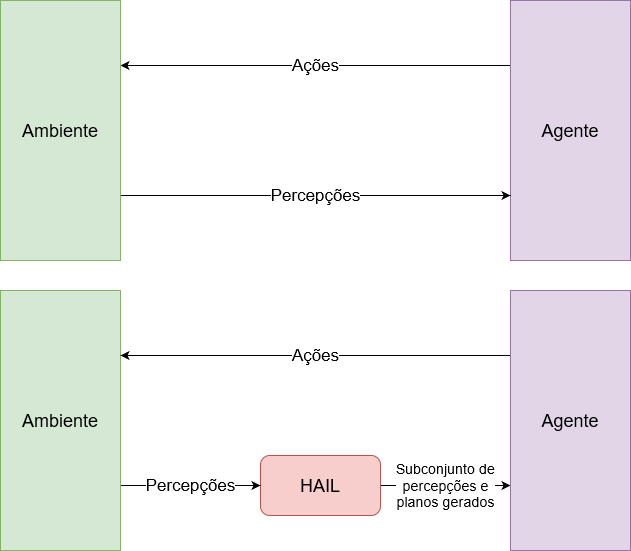
\includegraphics[width=\textwidth]{images/generalidade.png}
    \legend{Fonte: Autor}
    \label{fig:generalidade}
\end{figure}

O outro aspecto da generalidade do modelo diz respeito a sua alterabilidade. As principais partes modificáveis do HAIL são o módulo de revisão de percepções, o coeficiente de limpeza $\alpha$ utilizado pela função de limpeza dos blocos avaliadores e os blocos avaliadores.

O módulo de revisão de percepções pode ser implementado para utilizar qualquer técnica de refinamento de percepções, ou então não utilizar técnica alguma. Isso foi definido pois dependendo do tipo de ambiente no qual o agente está inserido pode ser necessário analisar todas as percepções recebidas ou filtrar de maneira bastante rígida quais percepções serão processadas.

O coeficiente de limpeza foi criado para que seja possível ajustar a frequência com a qual as listas ponderadas são limpas, tornando possível que agentes em situações com muitas anomalias não utilizem tanta memória e agentes em situações críticas possam analisar anomalias dentro de um maior período de tempo.

Por fim, o bloco de planejamento automatizado não teve uma estratégia ou arquitetura definida pois esse tipo de mecanismo é bastante complexo e não era o foco do trabalho. Além disso, como foi mostrado no Exemplo \ref{example::planejamento}, deixar a implementação do planejamento automatizado em aberto permite que o desenvolvedor adéque o modelo conforme a necessidade.